\documentclass[]{standalone}
\usepackage{tikz}
\usetikzlibrary{arrows,shapes,snakes,automata,backgrounds,petri}
\begin{document}
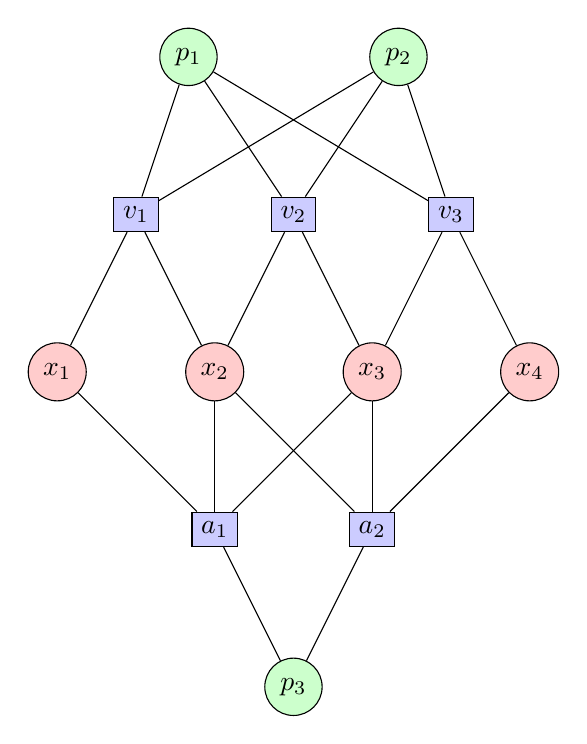
\begin{tikzpicture}[]
\node[draw, circle, fill=red!20] at (2.000000, 0.000000) (node0) {$x_{1}$};
\node[draw, circle, fill=red!20] at (4.000000, 0.000000) (node1) {$x_{2}$};
\node[draw, circle, fill=red!20] at (6.000000, 0.000000) (node2) {$x_{3}$};
\node[draw, circle, fill=red!20] at (8.000000, 0.000000) (node3) {$x_{4}$};
\node[draw, fill=blue!20] at (3.000000, 2.000000) (node4) {$v_{1}$};
\node[draw, fill=blue!20] at (5.000000, 2.000000) (node5) {$v_{2}$};
\node[draw, fill=blue!20] at (7.000000, 2.000000) (node6) {$v_{3}$};
\node[draw, fill=blue!20] at (4.000000, -2.000000) (node7) {$a_{1}$};
\node[draw, fill=blue!20] at (6.000000, -2.000000) (node8) {$a_{2}$};
\draw[] (node0) --  (node4);
\draw[] (node1) --  (node4);
\draw[] (node1) --  (node5);
\draw[] (node2) --  (node5);
\draw[] (node2) --  (node6);
\draw[] (node3) --  (node6);
\draw[] (node0) --  (node7);
\draw[] (node1) --  (node7);
\draw[] (node2) --  (node7);
\draw[] (node1) --  (node8);
\draw[] (node2) --  (node8);
\draw[] (node3) --  (node8);
\node[draw, circle, fill=green!20] at (3.666667, 4.000000) (node9) {$p_1$};
\node[draw, circle, fill=green!20] at (6.333333, 4.000000) (node10) {$p_2$};
\node[draw, circle, fill=green!20] at (5.000000, -4.000000) (node11) {$p_3$};
\draw[] (node9) --  (node4);
\draw[] (node10) --  (node4);
\draw[] (node9) --  (node5);
\draw[] (node10) --  (node5);
\draw[] (node9) --  (node6);
\draw[] (node10) --  (node6);
\draw[] (node11) --  (node7);
\draw[] (node11) --  (node8);
\end{tikzpicture}
\end{document}
